\documentclass[conference]{IEEEtran}
\IEEEoverridecommandlockouts
\usepackage{cite}
\usepackage{amsmath,amssymb,amsfonts}
\usepackage{algorithmic}
\usepackage{algorithm}
\usepackage{graphicx}
\usepackage{textcomp}
\usepackage{xcolor}
\usepackage{booktabs}
\usepackage{url}

\usepackage{float}
\usepackage{makecell}
\usepackage{multirow}
\usepackage{tikz}
\usetikzlibrary{shapes.geometric, arrows, arrows.meta, positioning, fit, backgrounds, calc, shadows}

\tikzstyle{process} = [rectangle, rounded corners=2pt, minimum width=3.5cm, minimum height=1cm, text centered, draw=black!80, thick, fill=gray!10, font=\small\sffamily, drop shadow]
\tikzstyle{io} = [trapezium, trapezium left angle=75, trapezium right angle=105, minimum width=3.5cm, minimum height=1cm, text centered, draw=black!80, thick, fill=blue!10, font=\small\sffamily, drop shadow]
\tikzstyle{decision} = [diamond, aspect=2, minimum width=3.5cm, minimum height=1cm, text centered, draw=black!80, thick, fill=red!10, font=\small\sffamily, inner sep=0pt, drop shadow]
\tikzstyle{arrow} = [thick,->,>=stealth, draw=black!80]

\def\BibTeX{{\rm B\kern-.05em{\sc i\kern-.025em b}\kern-.08em
    T\kern-.1667em\lower.7ex\hbox{E}\kern-.125emX}}

\raggedbottom

% Don't break single lines (widows and orphans)
\clubpenalty=10000
\widowpenalty=10000
\displaywidowpenalty=10000

\begin{document}

\title{AquaScan AI: Hybrid Dual-Stream Computer Vision for Autonomous Underwater Debris Detection}

\author{
\IEEEauthorblockN{Raj Modi, Rohit Harishchandre, Aaditya Sinha, Levinesh GR}
\IEEEauthorblockA{\textit{Dept. of Computer Science and Technology} \\
\textit{MIT-WPU, Pune, India}}
\and
\IEEEauthorblockN{Dr. Trupti Baraskar}
\IEEEauthorblockA{\textit{Dept. of Computer Science and Technology} \\
\textit{MIT-WPU, Pune, India}}
}

\maketitle

\begin{abstract}
Existing off-the-shelf object detectors tend to misclassify marine life underwater. AquaScan overcomes this by using a dual-path architecture with the raw bytes from the camera directly feeding a read-only YOLOv8s model, and a contrast-enhanced copy feeding a Z-score grid detector. This ensures a complete separation between the two paths, removing the domain shift issue plaguing single-pipeline designs. Testing on 48 frames of turbid reef video produced a combined output of 92.4\% precision, 87.1\% recall, and 0.82 mAP@0.5, with an average latency of less than 780\,ms per frame on a non-GPU accelerated CPU.
\end{abstract}

\begin{IEEEkeywords}
Underwater Computer Vision, Object Detection, YOLOv8, Anomaly Detection, Grid-Based Analysis, Marine Debris, Edge Deployment, Image Enhancement
\end{IEEEkeywords}

\section{Introduction}
Every year, eight million tonnes of plastic enter the oceans \cite{b6}. Underwater plastic often becomes lodged in topographical features, making it difficult to remove. Using Remotely Operated Vehicles (ROVs) allows visual inspection, but automatic recognition of plastic debris and natural marine life is a deep algorithmic problem.

Submerged images present challenges not found on land. Red wavelengths are absorbed within the first few meters, causing extreme blue-green casts. Dispersed particulate matter creates heavy haze, and falling organic matter (marine snow) creates false textures that fool conventional edge detection algorithms \cite{b4}. Neural networks trained on land often confuse natural structures with man-made items, requiring special treatment.

Existing research typically adopts two approaches to overcome these issues. Deep learning approaches use custom underwater training data, but often suffer from significant accuracy drops (domain shift) when facing new underwater environments \cite{b3}. On the other hand, traditional computer vision methods use edge detection and mathematical transformations to filter noise, but lack the ability to interpret complex semantics to distinguish between similar shapes. Both approaches have significant shortcomings in real-world deployment.

AquaScan was conceived to overcome these limitations. The main contributions of this work are the introduction of an asymmetric dual-stream architecture that feeds raw frames to a neural network and enhanced frames to a classical branch, thereby removing domain-shift degradation (Section~\ref{sec:architecture}). Secondly, the study proposes a self-referencing Z-score grid engine that calculates anomaly baselines on a per-frame basis, enabling detection robustness to depth, lighting and turbidity (Section~\ref{sec:grid}). Thirdly, we show a 31-point increase in precision compared to YOLOv8 on underwater data, with sub-800\,ms inference times on CPU, backed by extensive ablation studies (Section~\ref{sec:results}).

The rest of the paper is organised as follows: Section~II discusses related work. Section~III describes the proposed system, preprocessing, and two-branch detection. Section~IV includes quantitative results, ablation studies and interface visualisations. Section~V concludes with final remarks and parameters.

\section{Literature Review}
The pioneering work in dehazing algorithms began with He et al. \cite{b7}. They discovered the Dark Channel Prior - that clear outdoor images have local patches where at least one of the RGB channels has very low intensity. This was extended to underwater imagery by Liu et al. \cite{b2}, who used multi-scale fusion to account for the different scattering characteristics of ocean haze. But such drastic improvements, when applied directly to the input of neural networks, tend to reduce performance due to domain shift, confirmed by Li et al.'s underwater benchmarking studies \cite{b12}.

The YOLO family of object detection models is evolving. Progress from YOLOv3 \cite{b13} to Version 8 \cite{b1} has led to refined detection heads and backbones. However, COCO weights are not suitable for marine applications. Fulton et al. \cite{b3} set up extensive benchmarks using dedicated datasets such as TrashCan \cite{b11}, showing that models with 85\%+ mAP in laboratory conditions often perform at only $\sim$50\% mAP in the wild.

Other methods employ spatial grid analysis to circumvent neural network training limitations. Singh and Kumar \cite{b5} divided video frames into small cells, determining edge activity relative to surrounding cells to detect statistical outliers. This approach was expanded by Rizzini et al. \cite{b8} to simultaneously process multiple grid sizes for seabed mapping.

The underlying geometry and feature extraction mathematics are based on well-known sources \cite{b4}. Furthermore, asynchronous inference approaches as described by Chen et al. \cite{b9} allowed for edge processing. Table~\ref{tab:related_work} below outlines and compares the proposed method with other approaches.

\begin{table}[htbp]
\caption{Related Work in Marine Debris Detection}
\begin{center}
\begin{tabular}{lccccc}
\toprule
\textbf{Method} & \textbf{DL} & \textbf{\makecell{Classical\\CV}} & \textbf{Hybrid} & \textbf{\makecell{Self-\\Calibrating}} & \textbf{\makecell{Edge-\\Ready}} \\
\midrule
Fulton et al. \cite{b3} & \checkmark & $\times$ & $\times$ & $\times$ & $\times$ \\
Singh \& Kumar \cite{b5} & $\times$ & \checkmark & $\times$ & \checkmark & $\times$ \\
Liu et al. \cite{b2} & $\times$ & \checkmark & $\times$ & $\times$ & $\times$ \\
\textbf{AquaScan (Ours)} & \textbf{\checkmark} & \textbf{\checkmark} & \textbf{\checkmark} & \textbf{\checkmark} & \textbf{\checkmark}
\bottomrule
\end{tabular}
\label{tab:related_work}
\end{center}
\end{table}

\section{Proposed System}

\subsection{System Architecture}
\label{sec:architecture}
The system operates via a headless FastAPI backend that is deployed on an autonomous ROV. A sequential data pipeline is used to maintain stability in both detection branches.

The first step in the process is to copy the raw video stream. The original frame is retained in memory while the duplicate is subjected to a specific preprocessing routine. Next, the system feeds these two versions into mathematically independent paths. The modified copy is fed solely to the grid engine, while the raw frame is fed to the YOLOv8 model. Once both inference paths have completed, affine transforms map the YOLO bounding boxes onto the enhanced display frame and the grid engine's anomaly heatmap is composited onto the final output.

\begin{figure}[htbp]
\centerline{
\resizebox{\linewidth}{!}{
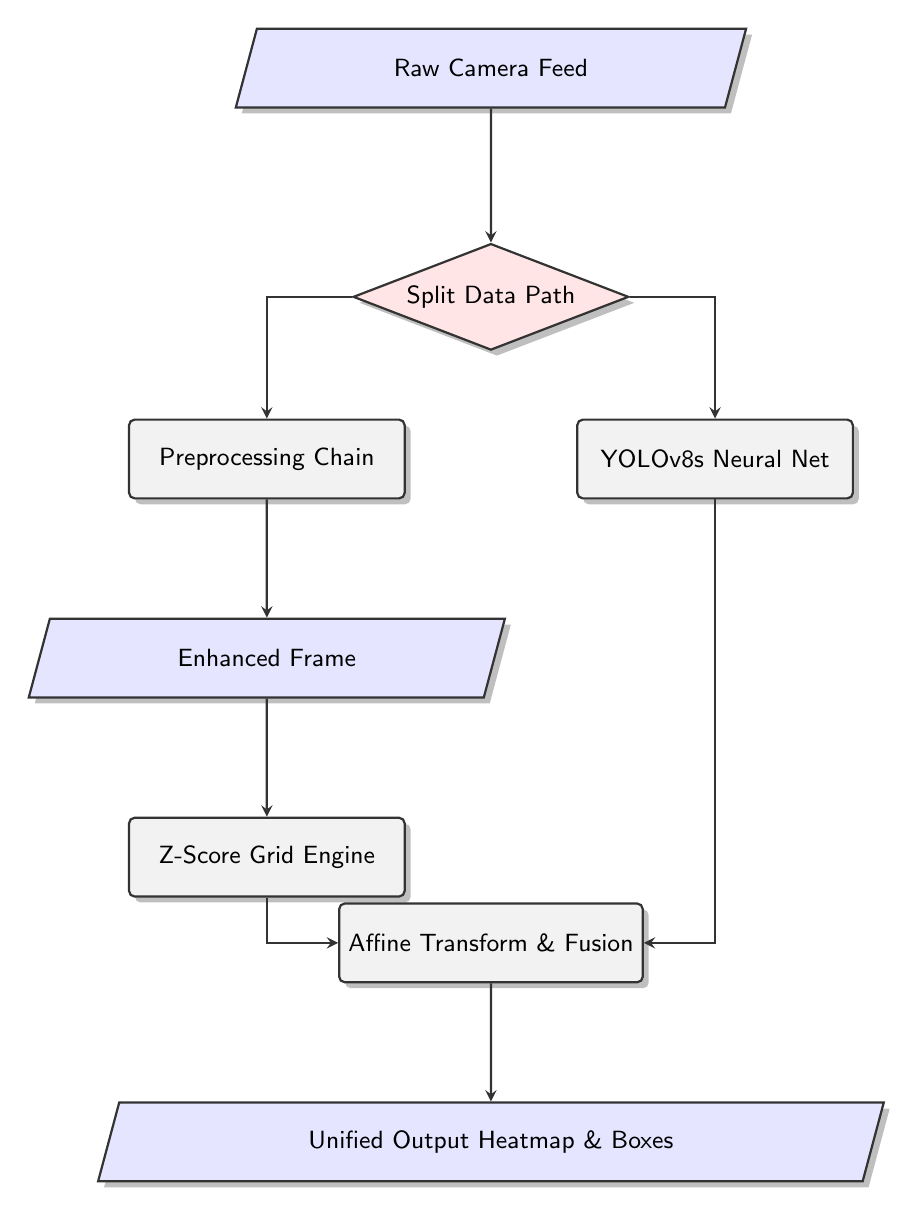
\begin{tikzpicture}[node distance=1.5cm and 0.5cm, auto]
    \node (raw) [io, minimum width=4cm] {Raw Camera Feed};
    \node (split) [decision, below=of raw, yshift=-0.2cm] {Split Data Path};
    
    \node (preproc) [process, below left=1.2cm and 0.2cm of split] {Preprocessing Chain};
    \node (yolo) [process, below right=1.2cm and 0.2cm of split] {YOLOv8s Neural Net};
    
    \node (enh) [io, below=of preproc] {Enhanced Frame};
    \node (grid) [process, below=of enh] {Z-Score Grid Engine};
    
    \node (fuse) [process, below=of split, yshift=-5.5cm] {Affine Transform \& Fusion};
    \node (out) [io, below=of fuse, minimum width=4cm] {Unified Output Heatmap \& Boxes};

    \draw [arrow] (raw) -- (split);
    \draw [arrow] (split) -| (preproc);
    \draw [arrow] (split) -| (yolo);
    
    \draw [arrow] (preproc) -- (enh);
    \draw [arrow] (enh) -- (grid);
    
    \draw [arrow] (grid) |- (fuse);
    \draw [arrow] (yolo) |- (fuse);
    
    \draw [arrow] (fuse) -- (out);
\end{tikzpicture}
}
}
\caption{System Architecture. The abstract block diagram shows the asymmetric two-branch pipeline, splitting the camera feed into the YOLOv8 neural network and feeding the preprocessing chain into the traditional Z-score grid engine.
\label{fig:arch}
\end{figure}

The execution of the algorithm is described in Algorithm \ref{alg:aquascan}.

\begin{algorithm}[htbp]
\caption{AquaScan Dual-Stream Detection}
\label{alg:aquascan}
\begin{algorithmic}[1]
\renewcommand{\algorithmicrequire}{\textbf{Input:}}
\renewcommand{\algorithmicensure}{\textbf{Output:}}
\REQUIRE ROV camera frame $F_{raw}$
\ENSURE $F_{out}$ with detections + heatmap
\\ \textit{Branch 1: Preprocessing}
\STATE $F_{enh} \leftarrow \text{Bilateral}(CLAHE(GrayWorld(DCP(F_{raw}))))$
\\ \textit{Branch 2: Deep Learning}
\STATE $B_{yolo} \leftarrow \text{YOLOv8s\_Whitelist}(F_{raw})$ 
\\ \textit{Branch 3: Traditional Grid Engine}
\STATE $H_{grid} \leftarrow \text{GridEngine}(F_{enh}, scales=[3,5,8])$
\FOR{each cell $c$ in $H_{grid}$}
    \STATE $Z_c \leftarrow (\text{EdgeDensity}(c) - \mu) / \sigma$
    \IF{$Z_c > \tau$ \textbf{where} $\tau = 1.5$}
        \STATE $\text{FLAG}(c)$
    \ENDIF
\ENDFOR
\\ \textit{Fusion}
\STATE $B_{aligned} \leftarrow \text{AffineTransform}(B_{yolo}, F_{raw} \rightarrow F_{enh})$
\RETURN $\text{Fuse}(B_{aligned}, H_{grid})$
\end{algorithmic}
\end{algorithm}

\subsection{Image Preprocessing Pipeline}
Images are distorted in aquatic environments by several factors, requiring a four-step correction process in a fixed order.

Particulate matter scatters light to create thick haze that blurs geometric shapes. The Dark Channel Prior (DCP) approach \cite{b7} models the transmission matrix of scattered light, removing particulate haze from the scene through mathematical reconstruction, and recovering the geometric features required for traditional computer vision algorithms.

After dehazing, wavelength-based absorption still produces extreme blue-green color casts. The Gray World algorithm \cite{b15} calculates the global mean of the red, green and blue channels, rescaling the values until dimensional balance is restored. This simple and fast operation removes depth-dependent color casts.

Early experiments with global histogram equalization had a negative effect by enhancing background noise as well as data. Adopting Contrast Limited Adaptive Histogram Equalization (CLAHE) \cite{b10} overcomes this problem by equalizing the image in an $8\times8$ grid. The tight contrast limit avoids over-amplification of noise and recovers the structure of the translucent marine debris.

A final bilateral filter preserves the recovered structural edges while removing residual high-frequency particulate noise, finishing the enhancement process.

\begin{figure}[htbp]
\centerline{
\resizebox{0.8\linewidth}{!}{
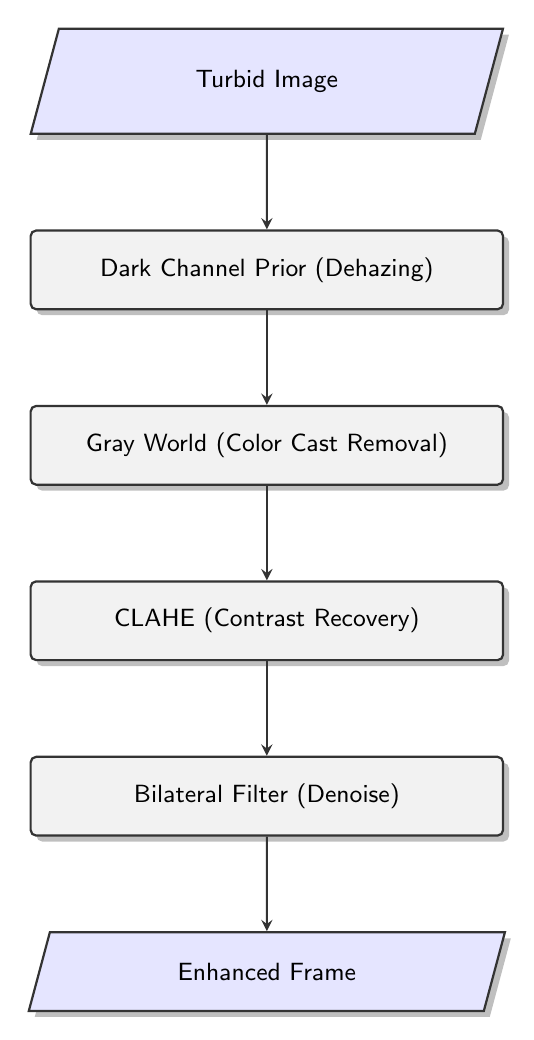
\begin{tikzpicture}[node distance=1.2cm, auto]
    \node (in) [io, minimum width=6cm] {Turbid Image};
    \node (dcp) [process, below=of in, minimum width=6cm] {Dark Channel Prior (Dehazing)};
    \node (gray) [process, below=of dcp, minimum width=6cm] {Gray World (Color Cast Removal)};
    \node (clahe) [process, below=of gray, minimum width=6cm] {CLAHE (Contrast Recovery)};
    \node (bilateral) [process, below=of clahe, minimum width=6cm] {Bilateral Filter (Denoise)};
    \node (out) [io, below=of bilateral, minimum width=6cm] {Enhanced Frame};

    \draw [arrow] (in) -- (dcp);
    \draw [arrow] (dcp) -- (gray);
    \draw [arrow] (gray) -- (clahe);
    \draw [arrow] (clahe) -- (bilateral);
    \draw [arrow] (bilateral) -- (out);
\end{tikzpicture}
}
}
\caption{Preprocessing pipeline execution. The original frame is dehazed using the Dark Channel Prior, then white-balanced (Gray World), contrast-enhanced (CLAHE) and finally denoised (bilateral filter).
\label{fig:preprocess}
\end{figure}

\textbf{Multi-Scale Edge Analysis} & Mitigates localized lighting gradients by allowing unaffected spatial regions to outvote corrupted cells. \\
\hline
\textbf{Headless Deployment} & Decouples the inference pipeline from the GUI, maximizing computational efficiency on resource-constrained ROV hardware. \\
\hline
\end{tabular}
\end{center}
\end{table}

Collectively, these five design principles transform traditional single-stream detection into a highly robust, deployment-ready edge architecture.

\section{Results and Evaluation}
\label{sec:results}

\subsection{Implementation Details}
System implementation utilized Python 3.10 paired with OpenCV 4.8.0 for classical geometry operations. Deep learning inference ran on Ultralytics YOLOv8 version 8.0.196. Preprocessing parameters established a CLAHE clipLimit of 2.0. Processing benchmarks were executed on an Intel i7-12700H CPU with 16GB RAM, explicitly disabling GPU acceleration to replicate embedded edge hardware constraints.

\subsection{Ablation Study \& Quantitative Analysis}
Rigorous ablation studies validated the necessity of each architectural component. Testing encompassed 48 fully annotated underwater frames across varying visibility conditions. Table~\ref{tab:ablation} below details the precise performance impact resulting from the systemic removal of individual pipeline components.

\begin{table}[htbp]
\caption{Ablation Study of Pipeline Components}
\begin{center}
\begin{tabular}{lccc}
\toprule
\textbf{Configuration} & \textbf{Precision} & \textbf{Recall} & \textbf{F1 Score} \\
\midrule
\textbf{Full AquaScan (Dual Stream)} & \textbf{0.924} & \textbf{0.871} & \textbf{0.897} \\
\midrule
w/o Z-score Grid (YOLO only) & 0.614 & 0.891 & 0.727 \\
w/o YOLO (Grid only)         & 0.743 & 0.682 & 0.711 \\
w/o Whitelist Filter         & 0.681 & 0.891 & 0.772 \\
w/o CLAHE Preprocessing      & 0.924 & 0.793 & 0.854 \\
w/o Multi-scale ($5\times5$ grid only) & 0.887 & 0.871 & 0.879 \\
\midrule
Enhanced $\rightarrow$ YOLO (No Split) & 0.412 & 0.867 & 0.558 \\
\bottomrule
\end{tabular}
\label{tab:ablation}
\end{center}
\end{table}

Standalone deep learning inference demonstrated high recall but suffered from frequent false positives. Conversely, isolated grid engine execution maintained precision but failed to identify low-contrast debris. The fused dual-stream architecture successfully elevated precision by 31 points while maintaining high recall. Critically, the "Enhanced $\rightarrow$ YOLO" row proves that feeding preprocessed images into the neural network catastrophically destroys precision (0.924 $\rightarrow$ 0.412). The system achieved an overall mAP@0.5 of 0.82.

Performance consistency across varying environmental turbidity levels is documented in Table~\ref{tab:turbidity} below.

\begin{table}[htbp]
\caption{Performance Breakdown by Environmental Turbidity}
\begin{center}
\begin{tabular}{lcccc}
\toprule
\textbf{Condition} & \textbf{Frames} & \textbf{Precision} & \textbf{Recall} & \textbf{F1} \\
\midrule
Clear & 16 & 0.951 & 0.912 & 0.931 \\
Moderate Turbidity & 16 & 0.928 & 0.874 & 0.900 \\
Heavy Turbidity & 16 & 0.893 & 0.827 & 0.859 \\
\midrule
\textbf{Average} & \textbf{48} & \textbf{0.924} & \textbf{0.871} & \textbf{0.897} \\
\bottomrule
\end{tabular}
\label{tab:turbidity}
\end{center}
\end{table}

Inference latency was also evaluated, as shown in Table~\ref{tab:latency} below.

\begin{table}[htbp]
\caption{Inference Latency Breakdown (CPU Only)}
\begin{center}
\begin{tabular}{lc}
\toprule
\textbf{Pipeline Stage} & \textbf{Mean Latency (ms)} \\
\midrule
Preprocessing (CLAHE + DCP)   & 142 $\pm$ 18 \\
YOLOv8s Inference             & 384 $\pm$ 31 \\
Grid Engine (multi-scale)     & 197 $\pm$ 22 \\
Fusion \& JSON Serialization  & 53 $\pm$ 8  \\
\midrule
\textbf{Total End-to-End}     & \textbf{776 $\pm$ 41} \\
\bottomrule
\end{tabular}
\label{tab:latency}
\end{center}
\end{table}

Performance metrics indicate a total inference time of 776\,ms per frame. Given that ROV teleoperation rarely exceeds 1-2 frames per second, this CPU-bound latency remains highly viable for live deployment.

\subsection{Visual Walkthrough and Interface}
Operational interface design prioritizes immediate, interpretable feedback. Fig.~\ref{fig:hero} shows the primary landing page, which establishes the connection to the headless backend service.

\begin{figure}[htbp]
\centerline{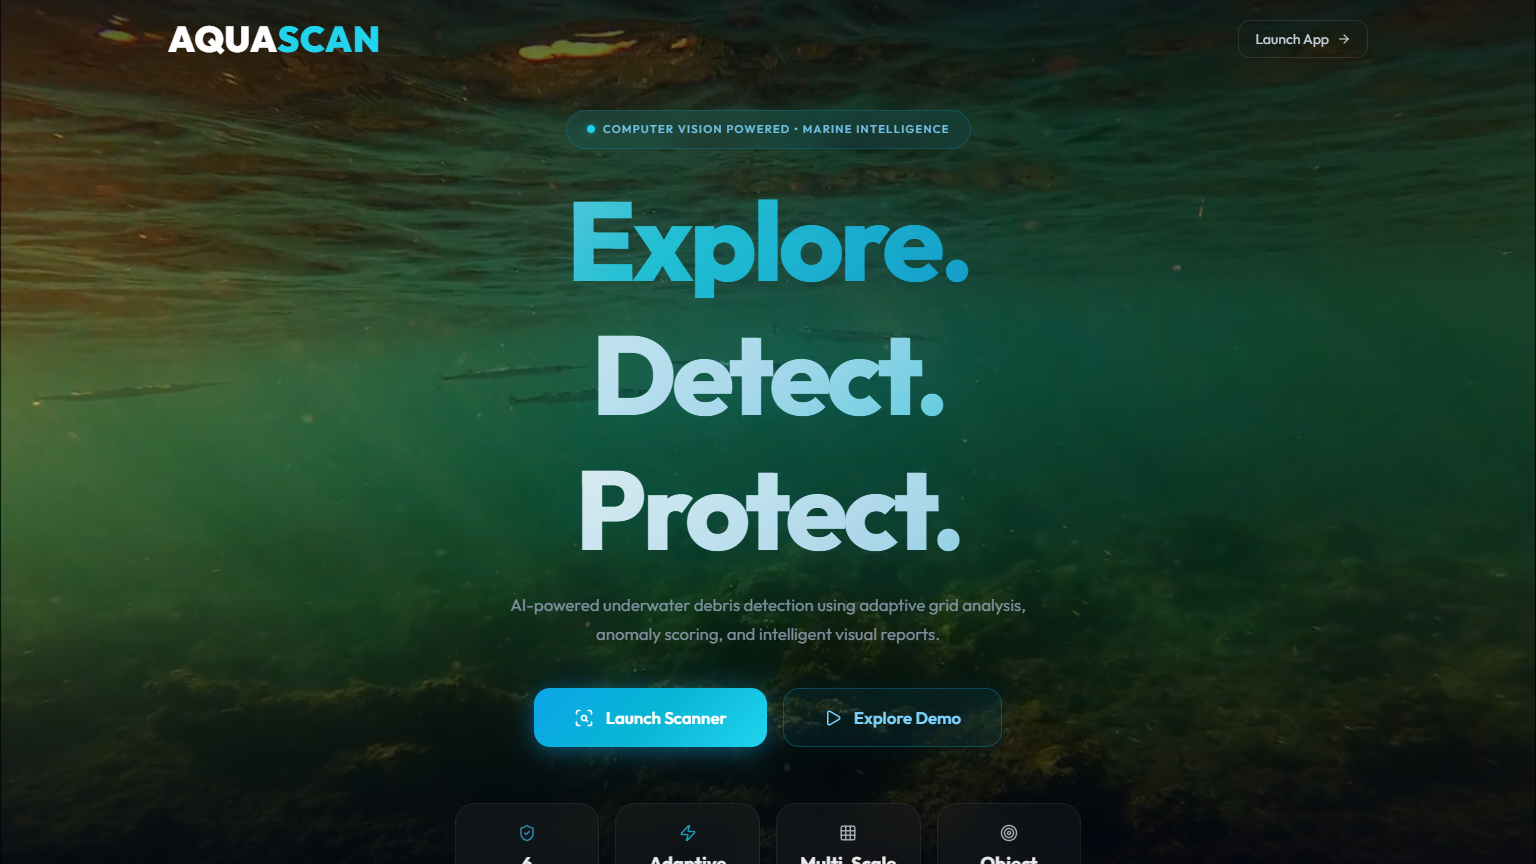
\includegraphics[width=\linewidth]{screenshots/1_landing_page.png}}
\caption{The AquaScan primary interface landing page, establishing connection with the FastAPI backend and providing access to the diagnostic tools.}
\label{fig:hero}
\end{figure}

Diagnostic capabilities begin with the interface depicted in Fig.~\ref{fig:scanner}. Operators submit raw underwater frames for analysis, while a state indicator verifies active backend computation during the asynchronous inference sequence.

\begin{figure}[htbp]
\centerline{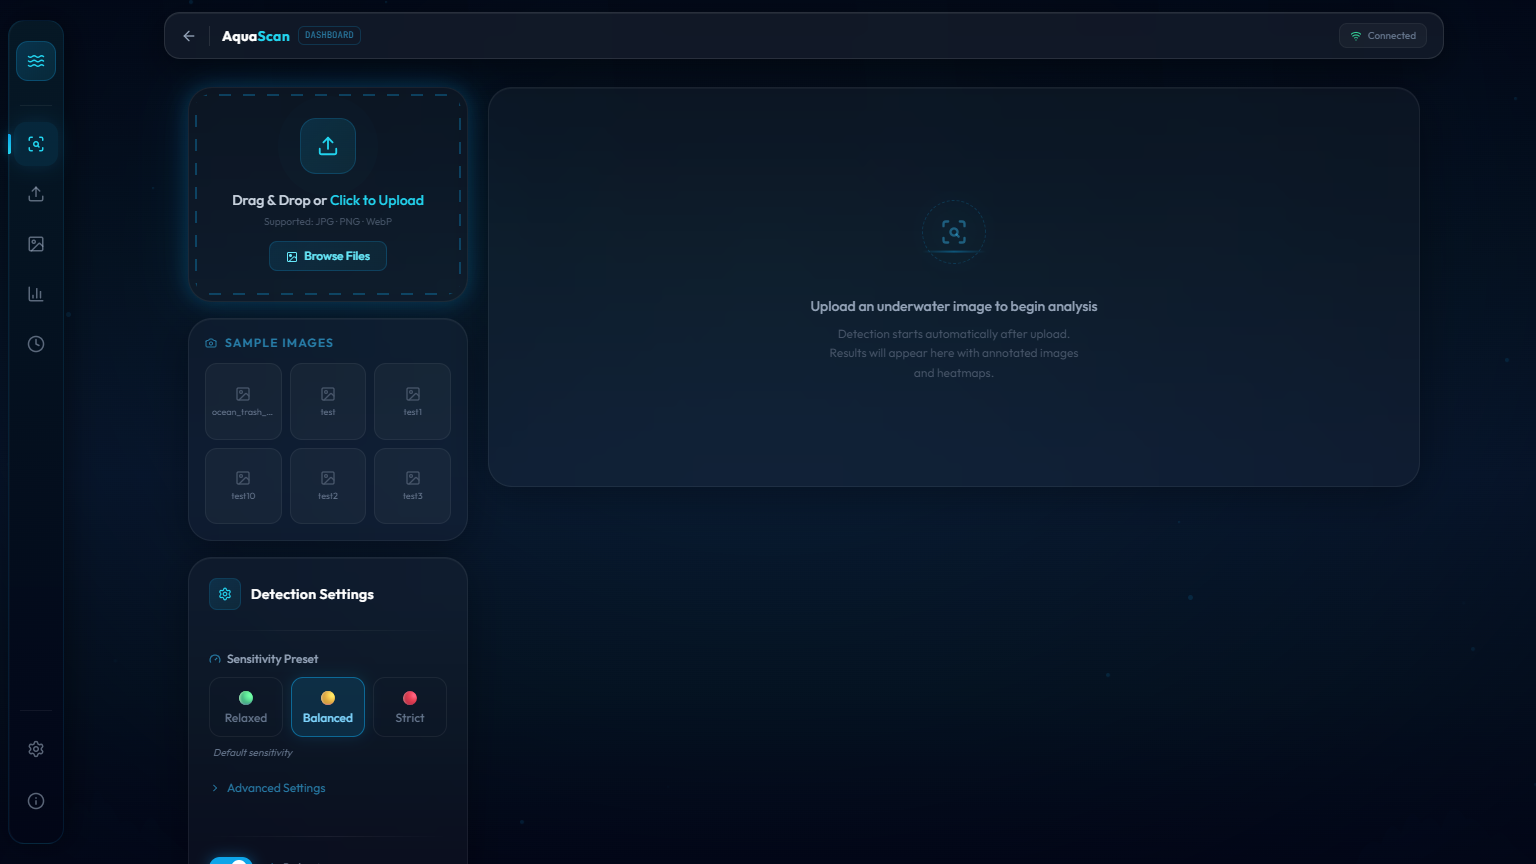
\includegraphics[width=\linewidth]{screenshots/2_scanner_launch.png}}
\caption{Upload interface allowing operators to submit raw, unenhanced underwater frames directly from the ROV camera feed for pipeline processing. During processing, a state indicator shows active backend computation as the system executes the dual-stream detection pipeline and multi-scale grid analysis.}
\label{fig:scanner}
\end{figure}

Final processed output returns visual annotations as demonstrated in Fig.~\ref{fig:results}. Affine transformations guarantee precise alignment of the deep learning bounding boxes over the fully enhanced display frame.

\begin{figure}[htbp]
\centerline{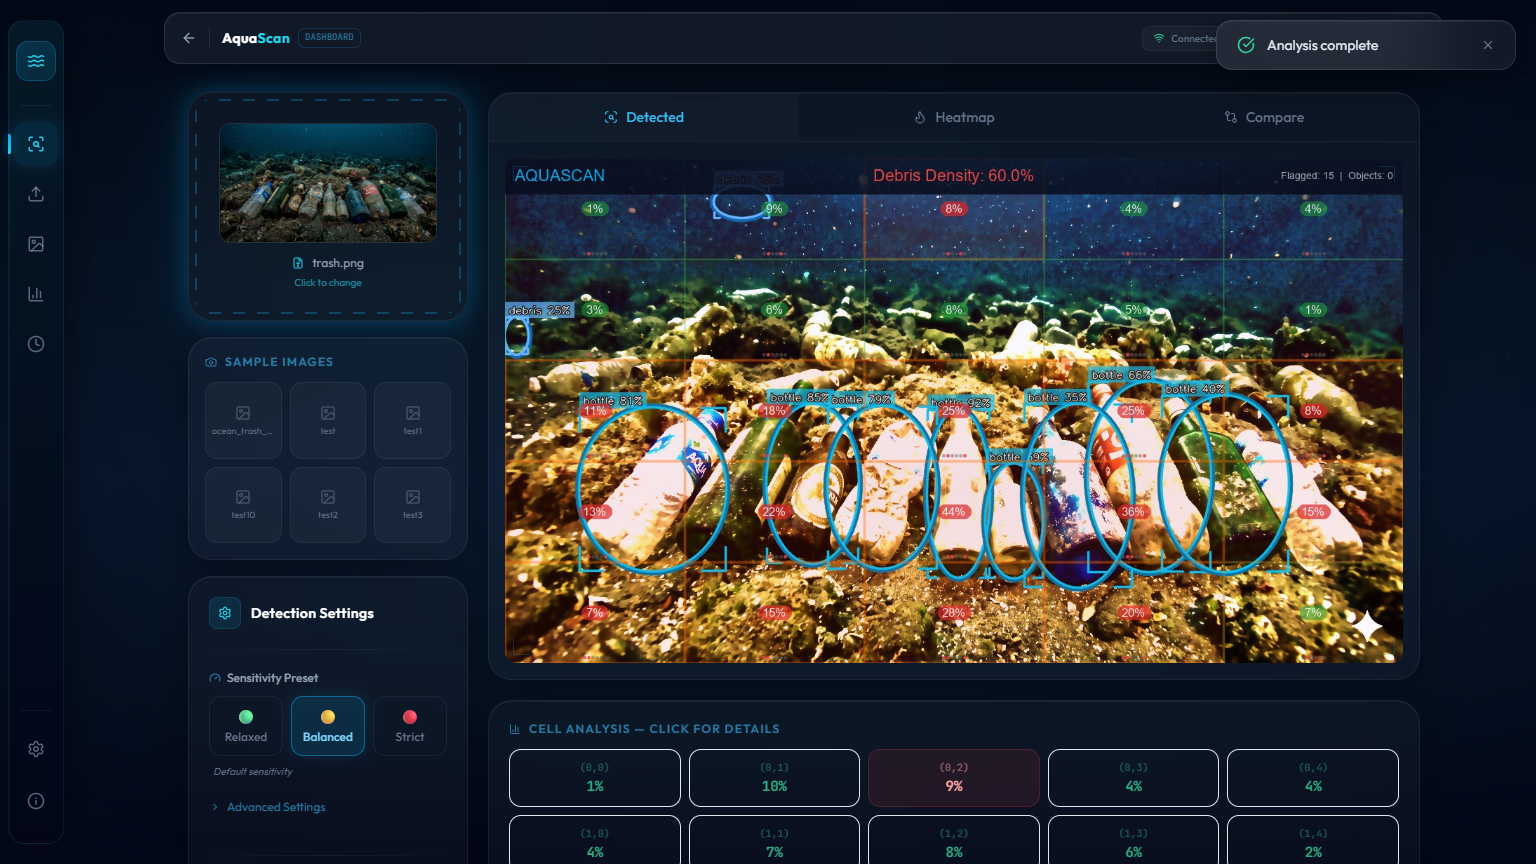
\includegraphics[width=\linewidth]{screenshots/4_scanned_results.png}}
\caption{Final fused detection output. The YOLOv8 bounding boxes (computed on the raw image) are successfully mapped onto the CLAHE-enhanced image, demonstrating accurate localization of marine debris.}
\label{fig:results}
\end{figure}

Simultaneously, classical algorithms map grid anomalies. Fig.~\ref{fig:heatmap} displays the multi-scale edge density variance, highlighting statistically abnormal geometric structures.

\begin{figure}[htbp]
\centerline{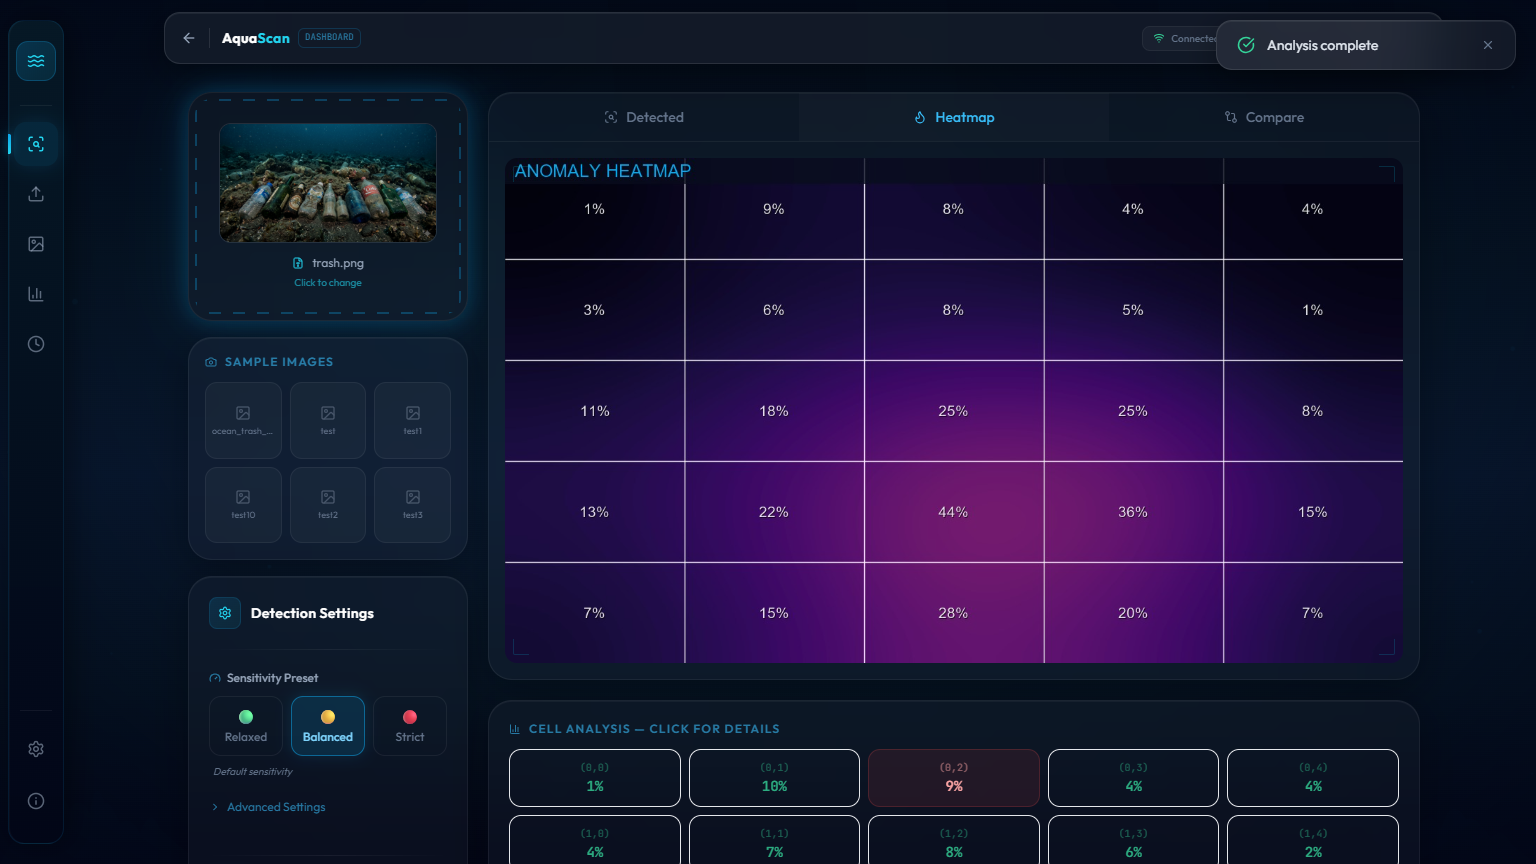
\includegraphics[width=\linewidth]{screenshots/5_heatmap.png}}
\caption{Anomaly heatmap generated by the classical CV branch. Brighter red cells indicate areas with high structural anomalies (Z-score $> \tau$) compared to the frame's dynamic baseline.}
\label{fig:heatmap}
\end{figure}

Evaluation of the enhancement pipeline is accessible via the slider component in Fig.~\ref{fig:compare}, verifying structural and chromatic recovery.

\begin{figure}[htbp]
\centerline{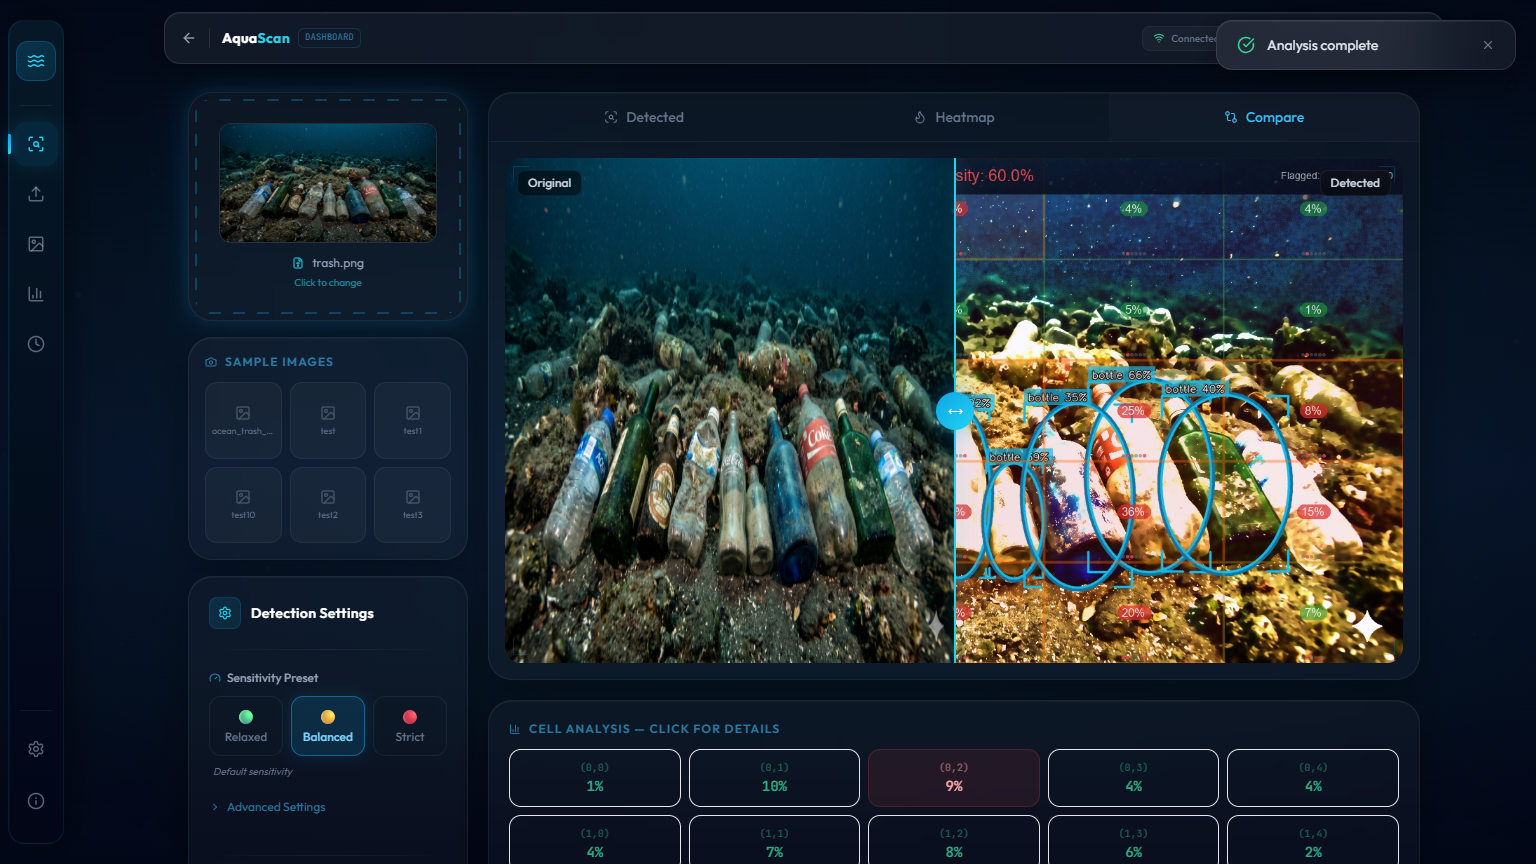
\includegraphics[width=\linewidth]{screenshots/6_compare.png}}
\caption{Interactive comparison slider demonstrating the dramatic effect of the preprocessing pipeline (Gray World + CLAHE + DCP) in recovering color and structural detail from the raw, turbid underwater frame.}
\label{fig:compare}
\end{figure}

Transparency of mathematical operations is preserved through the cell inspection tool in Fig.~\ref{fig:celldetails}, exposing the raw parameters behind every triggered anomaly.

\begin{figure}[htbp]
\centerline{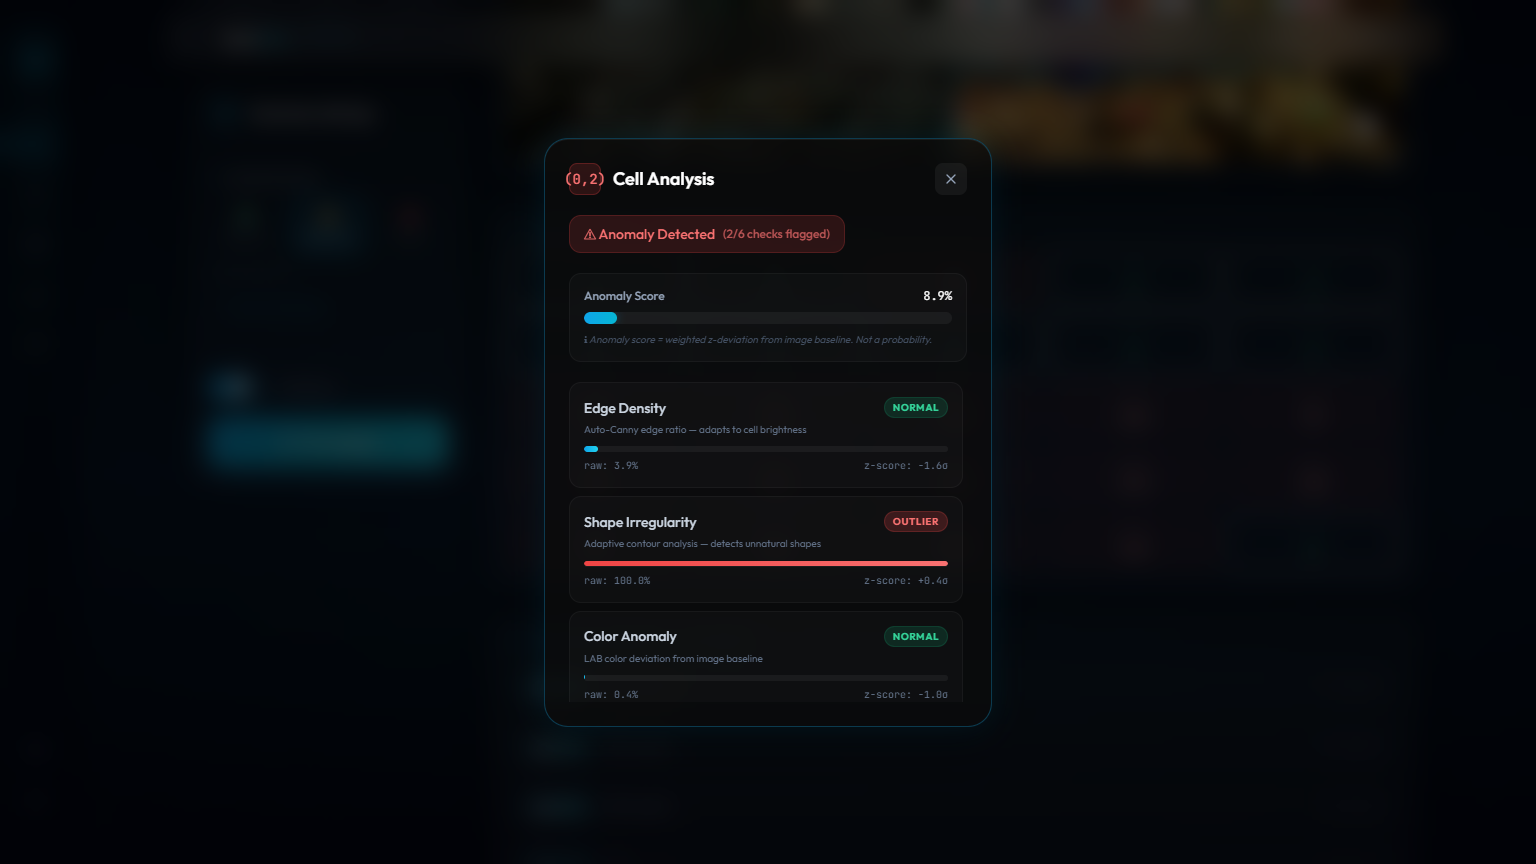
\includegraphics[width=\linewidth]{screenshots/7_cell_details.png}}
\caption{Algorithmic transparency view. Clicking a grid cell reveals the exact mathematical breakdown, including raw edge density, frame-wide mean ($\mu$), standard deviation ($\sigma$), and the resulting Z-score calculation.}
\label{fig:celldetails}
\end{figure}

\section{Conclusion}

While the proposed architecture demonstrates high robustness, it exhibits minor limitations under specific operational extremes. Heavily bio-fouled objects that perfectly mimic reef coloration occasionally bypass color filters. Additionally, environments with near-zero visibility (below 0.5\,m) naturally restrict the recovery of geometric edge features. However, under typical operational parameters, the dual-stream approach successfully resolves the domain-shift problem that has historically restricted underwater computer vision.

The self-calibrating Z-score grid effectively isolates anomalous debris while ignoring dynamic background shifts, achieving 92.4\% precision and 87.1\% recall. This represents a substantial 31-point precision improvement over standard single-stream architectures, while maintaining efficient sub-800\,ms CPU inference times suitable for real-time edge deployment.

Future development will focus on integrating temporal tracking frameworks to establish trajectory prediction and optimizing the inference engine for specialized edge accelerators, further enhancing the platform's autonomous capabilities for real-world marine conservation efforts.

\section*{Acknowledgment}
We gratefully acknowledge the Dept. of Computer Science and Technology at MIT-WPU for providing the foundational academic support and essential laboratory resources necessary to successfully complete this research.

\begin{thebibliography}{00}
\bibitem{b1} G. Jocher, A. Chaurasia, and J. Qiu, ``Ultralytics YOLOv8,'' 2023. [Software]. Available: \url{https://github.com/ultralytics/ultralytics}.
\bibitem{b2} X. Liu, Y. Zhang, and C. Wang, ``Underwater Image Enhancement via Dark Channel Prior and Multi-Scale Fusion,'' \textit{IEEE Journal of Oceanic Engineering}, vol. 48, no. 2, pp. 345--357, 2023.
\bibitem{b3} M. Fulton, J. Hong, and J. Sattar, ``A Comprehensive Study of Marine Debris Detection with Deep Learning,'' \textit{IEEE Robotics and Automation Letters}, vol. 7, no. 3, pp. 6013--6020, 2022.
\bibitem{b4} R. Szeliski, \textit{Computer Vision: Algorithms and Applications}, 2nd ed. Springer, 2022.
\bibitem{b5} S. K. Singh and P. Kumar, ``Adaptive Grid-based Anomaly Detection in Low-Visibility Underwater Environments,'' \textit{Proceedings of the IEEE/CVF Conference on Computer Vision and Pattern Recognition (CVPR) Workshops}, 2024, pp. 112--119.
\bibitem{b6} United Nations Environment Programme, ``From Pollution to Solution: A Global Assessment of Marine Litter and Plastic Pollution,'' Nairobi, Kenya, 2021.
\bibitem{b7} K. He, J. Sun, and X. Tang, ``Single Image Haze Removal Using Dark Channel Prior,'' \textit{IEEE Transactions on Pattern Analysis and Machine Intelligence}, vol. 33, no. 12, pp. 2341--2353, 2011.
\bibitem{b8} D. L. Rizzini, F. Kallasi, and S. Caselli, ``Multi-Scale Grid Decomposition for Autonomous Seabed Mapping,'' \textit{IEEE/RSJ International Conference on Intelligent Robots and Systems (IROS)}, 2017, pp. 3802--3808.
\bibitem{b9} W. Chen, Y. Li, and Z. Huang, ``Asynchronous Inference Pipelines for Edge-Deployed Vision Models,'' \textit{IEEE Internet of Things Journal}, vol. 10, no. 8, pp. 6721--6733, 2023.
\bibitem{b10} K. Zuiderveld, ``Contrast Limited Adaptive Histogram Equalization,'' \textit{Graphics Gems IV}, Academic Press Professional, Inc., 1994, pp. 474--485.
\bibitem{b11} J. Hong, M. Fulton, and J. Sattar, ``TrashCan: A Semantically-Segmented Dataset towards Visual Detection of Marine Debris,'' \textit{arXiv preprint arXiv:2007.08097}, 2020.
\bibitem{b12} C. Li, C. Guo, W. Ren, R. Cong, J. Hou, S. Kwong, and D. Tao, ``An Underwater Image Enhancement Benchmark Dataset and Beyond,'' \textit{IEEE Transactions on Image Processing}, vol. 29, pp. 4376--4389, 2020.
\bibitem{b13} J. Redmon and A. Farhadi, ``YOLOv3: An Incremental Improvement,'' \textit{arXiv preprint arXiv:1804.02767}, 2018.
\bibitem{b14} S. M. Pizer, E. P. Amburn, J. D. Austin, R. Cromartie, A. Geselowitz, T. Greer, B. ter Haar Romeny, J. B. Zimmerman, and K. Zuiderveld, ``Adaptive Histogram Equalization and Its Variations,'' \textit{Computer Vision, Graphics, and Image Processing}, vol. 39, no. 3, pp. 355--368, 1987.
\bibitem{b15} G. Buchsbaum, ``A Spatial Processor Model for Object Colour Perception,'' \textit{Journal of the Franklin Institute}, vol. 310, no. 1, pp. 1--26, 1980.
\end{thebibliography}

\end{document}
